\documentclass[msc,withpage,printonlyused]{yazd-thesis}
\usepackage{customization}
\usepackage{float}
\usepackage{multirow}
\usepackage{multicol}
\usepackage{intcalc}% http://ctan.org/pkg/calc
\usepackage{xepersian}

\settextfont[Scale=1.1]{Yas}
% فونت فرم صورت‌جلسه
\defpersianfont\minutesfont[Scale=1.2]{B Nazanin}
\setlatintextfont{Times New Roman} 
\setdigitfont[Scale=1]{Yas}
%\PersianMathsDigits
\SepMark{-}
\def\addsymbol #1:#2#3{$#1$ \> \parbox{5in}{#2 \dotfill \pageref{#3}}\\} 
\def\symboldisplay#1{\label{#1}} 

\begin{document}
	\baselineskip=1cm
	
\newword{minsupport}{MinSupport}{کمینه پشتیبان}{}
\newword{cosinesimilarity}{Cosine Similarity}{شباهت کسینوسی}{}
\newword{jaccard}{Jaccard}
{جاکارد}{}

	
	
	

	
	
	   \newcommand{\udate}[1]{
		\newcount\s
		\newcount\h
		\newcount\m
		\s=\intcalcNum {#1}
		%\s=\intcalcDiv{\s}{1000}
		\h=\intcalcDiv {\s} {3600}
		\s=\intcalcMod {\s} {3600}
		\m=\intcalcDiv {\s} {60}
		\s=\intcalcMod {\s} {60}
		\number\h:\number\m:\number\s
	}
	
	\newcommand{\rptable}[1]{
		%|c|c|c|c|c|c|c|c|c|c|
		\begin{tabular}{ c| c c c| c c c| c c c }
			\hline
			\multirow{2}{*}{}
			&
			\multicolumn{3}{c}{رویداد}
			&
			\multicolumn{3}{c}{عبارت}
			&
			\multicolumn{3}{c}{ میانگین عبارت رویداد}
			
			\\  
			
			
			\cline{2-10}
			
			&دقت&فراخوانی&\lr{F1}
			&دقت&فراخوانی&\lr{F1}
			&دقت&فراخوانی&\lr{F1}
			%		&
			%       			میانگین
			%	&
			%       			بیشینه
			%	&
			
			\\ 
			\hline
			
			#1
			\hline
		\end{tabular}
		
	}
	\newcommand{\ptable}[1]{
		\def\arraystretch{1.5}
		\begin{tabular}{ c| c c |c }
			\hline
			\multirow{2}{*}{}
			&
			\multicolumn{2}{c|}{حافظه (MB)}
			&
			\multirow{2}{*}{زمان}
			\\  
			
			
			\cline{2-3}
			&
			میانگین
			&
			بیشینه
			&
			
			\\ 
			\hline
			#1
		\end{tabular}
		
	}
	\newcommand{\results}[2]{
		\begin{figure}[H]
			\begin{center}
				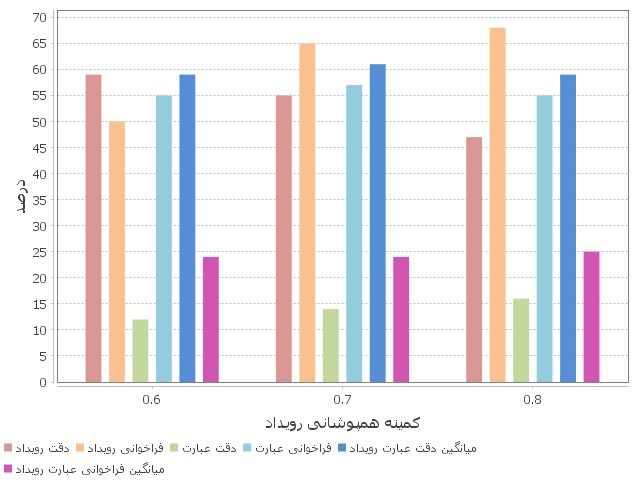
\includegraphics[width=0.7\textwidth]{train/#1/pic1}
				\caption{نمودار دقت و فراخوانی برای انتخاب پارامتر 
					#2}\label{fig1#1}
			\end{center}
		\end{figure}
		\begin{figure}[H]
			\begin{center}
				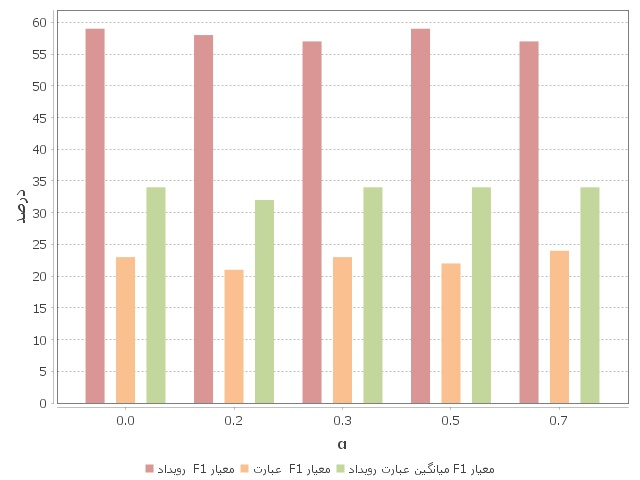
\includegraphics[width=0.7\textwidth]{train/#1/pic2}
				\caption{نمودار \lr{F1}  برای انتخاب پارامتر 
					#2}\label{fig2#1}
			\end{center}
		\end{figure}
		
		
		
		\begin{table}[H]
			\begin{center}
				\def\arraystretch{1.5}
				%	 \captionof{table}{جدول دقت و فراخوانی برای انتخاب پارامتر 
				%	 	#2}\label{tab1#1}
				\caption{جدول دقت و فراخوانی برای انتخاب پارامتر 
					#2}\label{tab1#1}
				\rptable{$0.0$ &$ 53.9 $ &$ 64.9 $ &$ 58.9 $ &$ 14.1 $ &$ 55.2 $ &$ 22.5 $ &$ 59.4 $ &$ 23.8 $ &$ 34.0 $ \\ 
  \hline  
 $0.2$ &$ 52.8 $ &$ 63.5 $ &$ 57.7 $ &$ 13.0 $ &$ 53.8 $ &$ 21.0 $ &$ 58.1 $ &$ 22.4 $ &$ 32.4 $ \\ 
  \hline  
 $0.3$ &$ 51.6 $ &$ 64.9 $ &$ 57.5 $ &$ 14.5 $ &$ 56.5 $ &$ 23.1 $ &$ 59.8 $ &$ 24.1 $ &$ 34.3 $ \\ 
  \hline  
 $0.5$ &$ 53.3 $ &$ 66.2 $ &$ 59.0 $ &$ 13.8 $ &$ 54.2 $ &$ 22.0 $ &$ 58.8 $ &$ 23.5 $ &$ 33.6 $ \\ 
  \hline  
 $0.7$ &$ 51.1 $ &$ 64.9 $ &$ 57.1 $ &$ 15.1 $ &$ 55.2 $ &$ 23.7 $ &$ 59.0 $ &$ 24.2 $ &$ 34.4 $ \\ 
  \hline  
 }
			\end{center}
		\end{table}
		
		
		\begin{table}[H]
			\begin{center}
				%	 \captionof{table}{جدول کارایی برای انتخاب پارامتر 
				%	 	#2}\label{tab2#1}
				\caption{جدول کارایی برای انتخاب پارامتر 
					#2}\label{tab2#1}
				\def\arraystretch{1.5}
				\ptable{$0.0$ &$ 682.2 $ &$ 1483.0 $ &$\udate{5742}$  \\ 
  \hline  
 $0.3$ &$ 714.6 $ &$ 1511.0 $ &$\udate{5740}$  \\ 
  \hline  
 $0.5$ &$ 775.6 $ &$ 1522.0 $ &$\udate{5708}$  \\ 
  \hline  
 $0.7$ &$ 662.0 $ &$ 1397.0 $ &$\udate{5786}$  \\ 
  \hline  
 }
			\end{center}
		\end{table}
	}
	
	\newcommand{\bitem}[2]{
%		\item 
		\section{#1}:
		
		#2}
	
	\newcommand{\result}[2]{
\bitem{#2}{\results{#1}{#2}}	
}
	
	
	
	
	
	\chapter{نتایج}

	



\result{minsupport}{\gls{minsupport}}
		\result{delta}{$\delta$}
		\result{jacTH}{آستانه‌ی \gls{jaccard}}
		\result{MinCosinSim}{کمینه \gls{cosinesimilarity}}
		\result{k_knn}{$k\_KNN$}
		\result{a}{$\alpha$}
		\result{gs_k}{$\rho$}
		\result{b}{$\beta$}
		\result{ch}{$\tau$}
		\result{ne}{$\eta$}
		\result{K_TopScoreKeyword}{K عبارت برتر }
		\result{K_TopPattern}{K الگوی برتر}	
		\result{Min_keyword_count}{کمینه تعداد عبارت رویداد}
		\result{Min_topic_overlap}{کمینه همپوشانی رویداد}

	
\end{document}